\chapter{Sensors and Equipment}
I have 5 sensors, 1GSM-GPRS modem, 1 arduino mega and power supply. All the equipment are shown in below table:\newline
\begin{table}[h!]
\begin{center}
\begin{tabular}{|c|c|c|}
  \hline
  No. & Equipment Name & Model \\
  \hline
  1 & Temperature Sensor & LM35  \\
  \hline
  2 & Gas Sensor & MQ6  \\
  \hline
  3 & Carbon Monoxide Sensor & MQ9  \\
  \hline
  4 & Humidity Sensor & DHT11  \\
  \hline
  5 & Noise Sensor & KY-038  \\
  \hline
  6 & GPS GSM GPRS Module & SIM900  \\
  \hline
\end{tabular}{}
\end{center}
\caption{Sensors and other equipments}
\label{table:}
\end{table}
\section{Temperature Sensor}
It is an electronic device that measures the temperature of it's environment and converts the input data into electronic data to record, monitor, or signal temperature changes. Here, I have used LM35 sensor. LM35 can Measure the temperature of a particular environment, provide thermal shutdown for a circuit/component, monitor battery temperature, measuring temperatures for HVAC applications. It has 3 pin. One pin is for 4-20 volt input, another is out pin and another is for ground. \cite{liu2011application}
\begin{figure} [h!]
\centering
 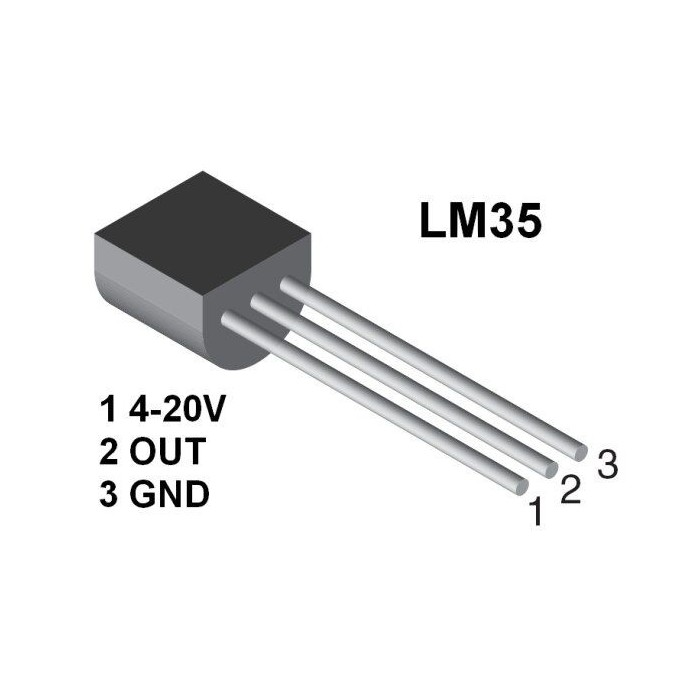
\includegraphics[width=10cm]{Results/lm35.jpg}
 \caption[]{LM35 Temperature Sensor}
    \label{}
\end{figure}
\section{Gas Sensor}
It is an electronic device that is used to detect toxic or explosive gasses and measure gas concentration.. Here, I have used MQ6 sensor. The MQ6 can be used in gas leakage detecting equipment in consumer and industry applications,this sensor is suitable for detecting LPG, iso-butane, propane, LNG. It is consists of a sensing element which comprises of the following parts \cite{evalina2020use}.
\begin{enumerate}[i]
    \item Gas sensing layer
    \item Heater Coil
    \item Electrode line
    \item Tubular ceramic
    \item Electrode
\end{enumerate}
\begin{figure} [h!]
\centering
 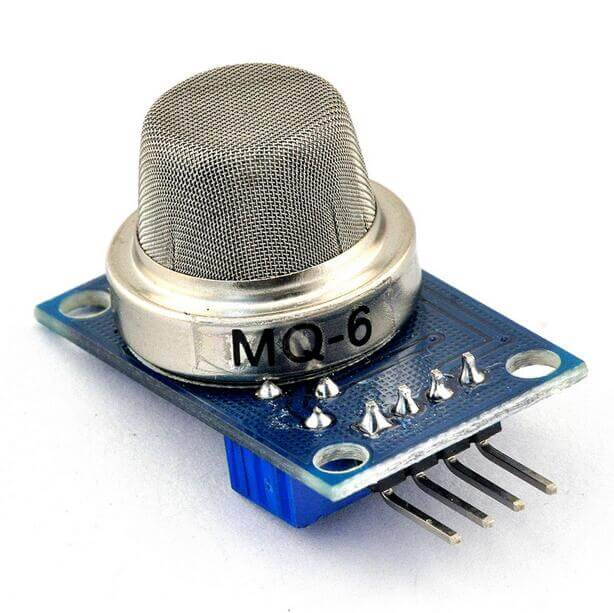
\includegraphics[width=7cm]{Results/MQ6.jpg}
 \caption[]{MQ6 Gas Sensor}
    \label{}
\end{figure}
\section{Carbon Monoxide Sensor}
I have used MQ9 sensor as $CO$ sensor. The MQ-9 Analog Gas Sensor has high sensitivity to Carbon Monoxide, Methane and LPG.\cite{setiawan2018iot}
\begin{figure} [h!]
\centering
 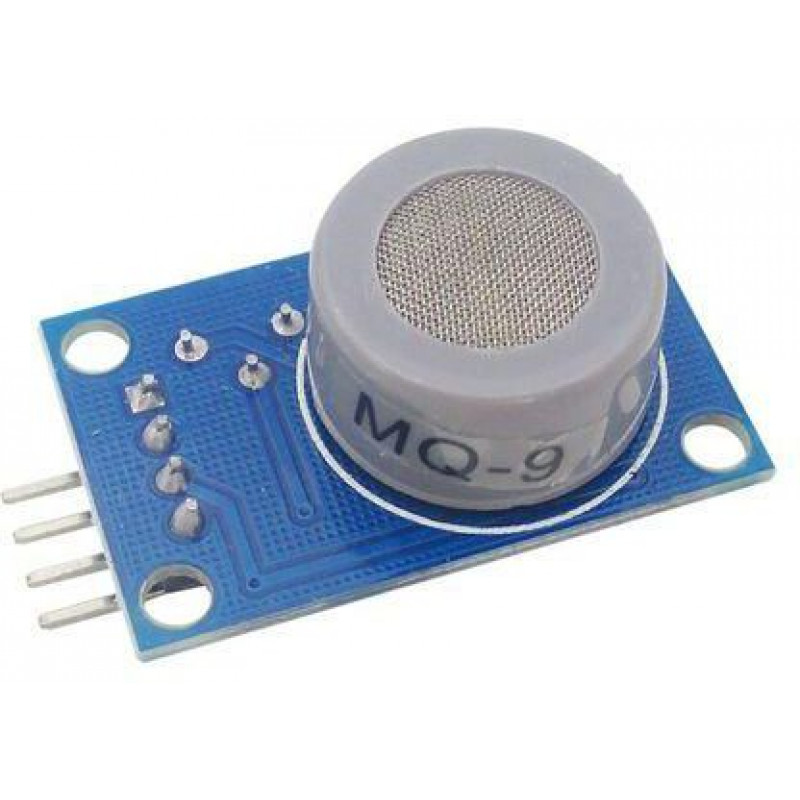
\includegraphics[width=7cm]{Results/mq9.jpg}
 \caption[]{MQ9 $CO$ Sensor}
    \label{}
\end{figure}
\section{Humidity Sensor}
A humidity sensor is an electronic device that measures the humidity in its environment and converts its findings into a corresponding electrical signal. I have used HDT11 as hunidity sensor. It senses, measures and reports both moisture and air temperature. Humidity sensors work by detecting changes that alter electrical currents or temperature in the air.\cite{kuang2007high}
\begin{figure} [h!]
\centering
 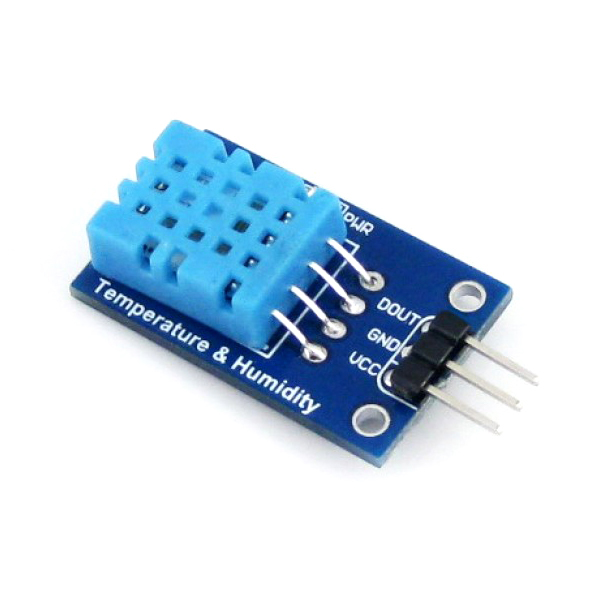
\includegraphics[width=7cm]{Results/hdt111.jpg}
 \caption[]{HDT11 Humidity Sensor}
    \label{}
\end{figure}
\section{Noise Sensor}
I have used KY038 sensor as noise sensor. It sensor is a very basic sound level detector module which features an electric condenser microphone. It is part of a sensor kit that can be purchased and the main part of the module is an LM393 cooperator. \cite{chen2008determining}
\begin{figure} [h!]
\centering
 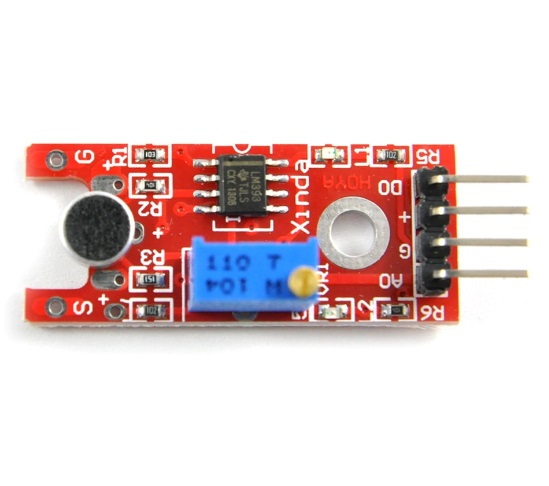
\includegraphics[width=7cm]{Results/ky038.jpg}
 \caption[]{KY038 Noise and Sound Sensor}
    \label{}
\end{figure}
\section{Arduino}
I have used Arduino Mega as micro-controller. The Arduino Mega 2560 is a micro-controller board based on the ATmega2560. It has 54 digital input/output pins (of which 15 can be used as PWM outputs), 16 analog inputs, 4 UARTs (hardware serial ports), a 16 MHz crystal oscillator, a USB connection, a power jack, an ICSP header, and a reset button.\cite{barrett2013arduino}
\begin{figure} [h!]
\centering
 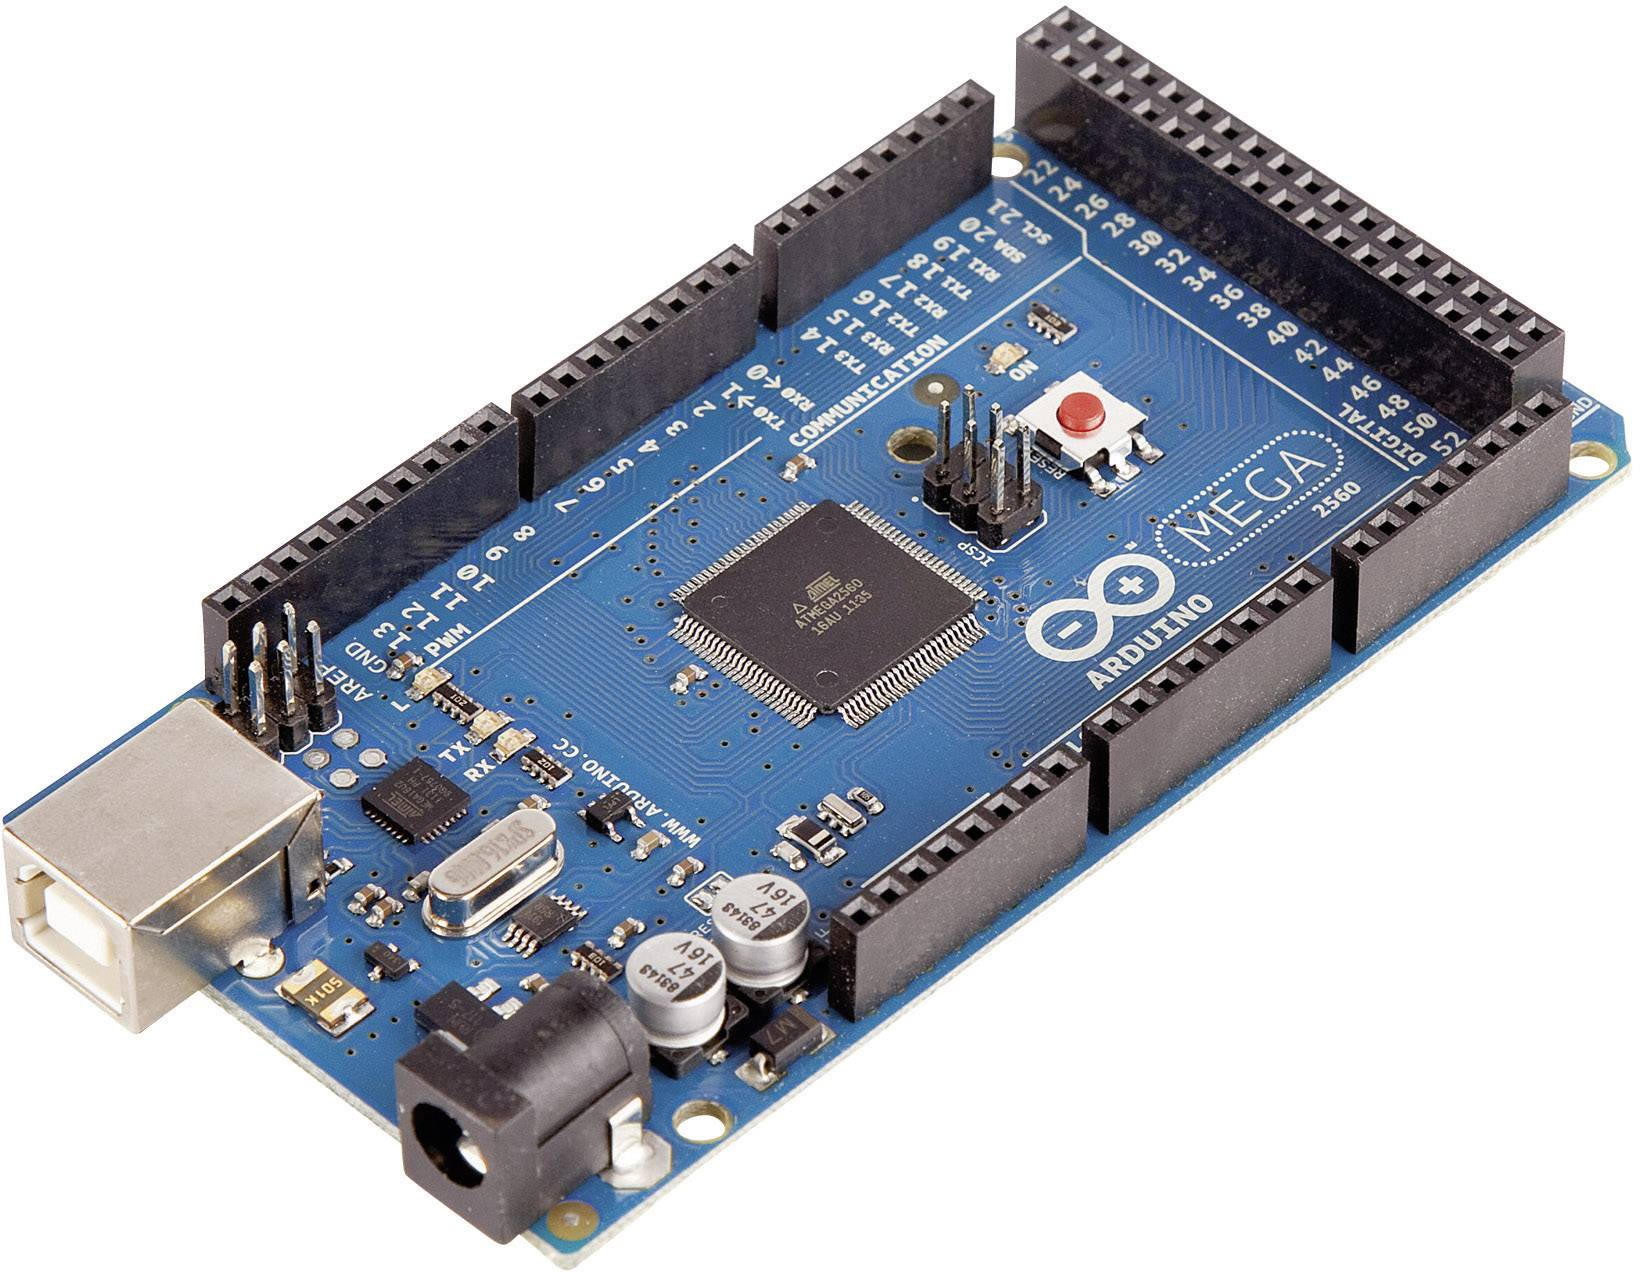
\includegraphics[width=6cm]{Results/arduino.jpg}
 \caption[]{Arduino Mega}
    \label{}
\end{figure}
\section{GPS GSM GPRS Module}
The SIM900 is a complete Quad-band GSM/GPRS solution in a SMT module which can be embedded in the customer applications. ... With a tiny configuration of 24mm x 24mm x 3 mm, SIM900 can fit almost all the space requirements in your M2M application, especially for slim and compact demand of design.\cite{leekongxuesmart}
\begin{figure} [h!]
\centering
 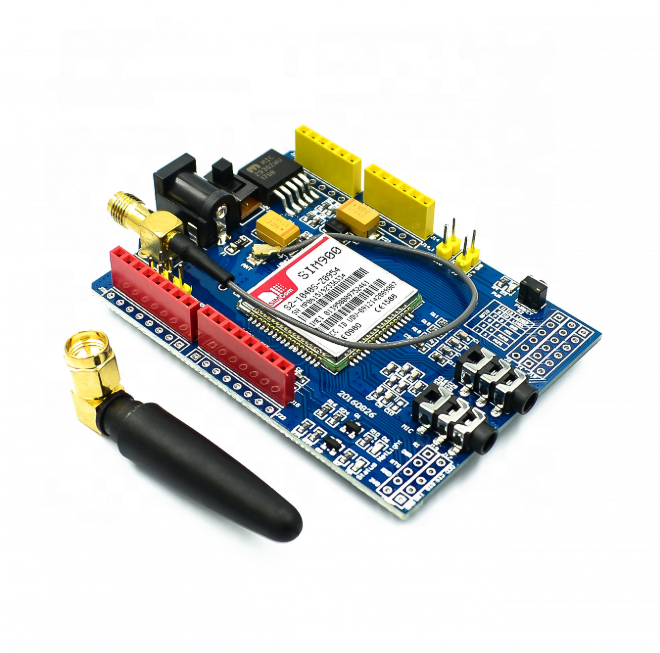
\includegraphics[width=5cm]{Results/900.png}
 \caption[]{GPS GSM GPRS Module}
    \label{}
\end{figure}